\chapter{統計学の基礎}
\label{chap_Statistics}

実験データの解析作業の目的のひとつは、何らかの物理量をそこから抽出し、その値が統計学的にどれだけ正しいかを評価することです。例えば電子の質量が約511~keVであることを私たちは知っていますが、その真の値がいくつかは誰も知りません\footnote{光速$c$のように299~792~458~$\mathrm{m}/\mathrm{s}$と正確に「定義」されている物理量も存在します。}。物理実験から統計学的な表現で言えるのは、電子質量は
\begin{equation}
  m_\mathrm{e} = 510.998\,946\,1\pm0.000\,003\,1\,\mathrm{keV}
\end{equation}
ということだけです\cite{Patrignani:2016:Review-of-Particle-Physics}。これは510.998~946~1~keVがこれまでの実験でわかった最も良い電子質量の推定値であり、その誤差は0.000~003~1~keVである、もしくは言い方を変えると、約68\%の確率\footnote{より正確には約$68.27$\%であり、これは正規分布の$\pm1\sigma$の範囲に入る確率です。この意味については本章で後述します。}で0.000~003~1~keVの範囲に収まっているという意味です。

ROOTではヒストグラムが自動で計算する平均値や標準偏差といった数値を始めとして、カイ二乗フィットや検定など、様々な統計処理が現れます。これらを理解せずにROOTを使ったりデータ解析を行うと、間違った物理量やその誤差を導出する恐れがありますし、また論文を読んでいても実験データの解釈を正しくできないでしょう。

実験系高エネルギー宇宙物理学の大学院生が必要とする統計学の基本的な情報、またそれをROOTでどのように扱えば良いかをこの章では説明します。

\section{参考書}

この章では非常に基本的なことしか触れませんし、その目的は統計学を学ぶことではなく、ROOTでどのように統計学的な考え方をするかの指針を与えることです。統計学、特に素粒子物理学や宇宙物理学で重要となる統計処理に関しては、いくつかの参考書を挙げるにとどめます。

\begin{enumerate}
  \item \myhref{http://pdg.lbl.gov}{C.~Patrignani and Particle Data Group, ``Review of particle physics'',  {\em Chinese Physics C} {\bf 40}, 100001 (2016)}\\
    素粒子物理学の研究者が2年ごとに編纂している、無料で入手可能な書籍です。この本の確率と統計の章は短いですがよくまとまっています。
  \item \myhref{http://amzn.to/2rzflO2}{Olaf Behnke et~al.``Data Analysis in High Energy Physics: A Practical Guide to Statistical Methods'', Wiley-VCH (2013)}\\
    比較的最近の本で、unfoldingや系統誤差の取り扱い、また天文学での事例など多岐にわたり解説しています。
  \item \myhref{http://amzn.to/2rg6gtJ}{Louis Lyons, ``Statistics for Nuclear and Particle Physicists'', Cambridge University Press, (1989)}\\
    古くからある素粒子・原子核物理向けの統計の教科書です。指導教員の多くが薦めると思います。
  \item \myhref{http://amzn.to/2rg6EIv}{Glenn F. Knoll, ``Radiation Detection and Measurement'', Wiley, 4th edition, (2010)}\\
    放射線計測に関する様々な情報が載っている教科書ですが、簡単な統計の話も取り扱っていて簡単に読めます。
\end{enumerate}

\section{基本的な用語}

\subsection{統計誤差と系統誤差}

一般的に測定値には誤差がつきます。例えばある放射性同位体の放射能を測定することを考えてみましょう。10秒間に100回の崩壊が計数されたとすると、この放射性同位体は10~Bq(ベクレル\footnote{1秒間に平均$N$回崩壊する放射性同位体の放射能を$N$~Bqと表します。})だと言えます。しかしこれは10秒間で崩壊した数がたまたま100回だっただけであり、繰り返し測定を行うと110回だったり90回だったりする可能性もあります。したがって我々が決定できる10~Bqというのはその測定における最良の推定値であり、確率に基づいた誤差が伴います。これを\emphasize{統計誤差(statistical error)}と呼びます。

この例の場合、原理的には測定時間を無限に長くすることで、統計誤差を限りなく小さくすることができます。しかし無限の測定時間を使うことは不可能であり、またその間に放射能自体が変化してしまいます。我々はあらゆる実験において、限られた時間、限られた装置、限られた金銭的・人的資源を使うことしかできませんので、必ず統計誤差と付き合うことになります。

一方、10秒間の測定と簡単に言っても、10秒間を精確に決めるのは困難です。使っている時計が原子時計でもない限り、多少のずれは必ず発生します。10秒間だと思って計測していても、実際には9.9秒だったり10.1秒だったりと、測定系自体に狂いが存在する可能性があります。この場合、10~Bqという推定値は、本当は10.1~Bqだったり9.9~Bqだったりするかもしれません。このような測定系自体の持つ誤差を\emphasize{系統誤差(systematic error)}と呼びます。

例えば上述の時計の場合、時計がどの程度ずれているかというのを、何かしらの外部装置を使って較正し、系統誤差を評価する必要があります。数学の計算さえ間違えなければ、一般的にはあらゆる実験で統計誤差を計算することが可能ですが、系統誤差の評価方法には王道は存在せず、それを解説した書籍も多くないでしょう。本書でも系統誤差については解説しませんので、各実験ごとの系統誤差の評価は、指導教員や先輩に相談しましょう。

\subsection{母集団と標本}

カミオカンデ実験の検出した超新星SN~1987Aからの11個のニュートリノは、SN~1987Aから放出された全てのニュートリノではありません。大マゼラン雲から地球の方向へ飛んできたニュートリノのうち、たまたまカミオカンデで検出された11個に過ぎません。我々は地球上に住んでいるため、SN~1987Aで発生した全方向のニュートリノを観測することはできませんし、また検出器の体積にも限りがあるため、地球に飛来した全てのニュートリノを検出することはできません。

このように物理実験では、発生した全ての事象を観測することができず、その一部だけを観測することによって物理量(例えばこの場合は超新星爆発のエネルギーがニュートリノにどれだけ渡されるかなど)を測定することが多々あります。この一部分のことを\emphasize{標本(sample)}と呼び、それに含まれる事象の数を\emphasize{標本の大きさ(sample size)}と呼びます\footnote{「標本数」(the number of samples)と誤用されることがありますが、これは用語として正しくありません。カミオカンデの他にIMB実験とBaksan実験でもニュートリノが同時に検出されており、標本は合計で3つあることになります。このとき、標本数は3であると言います。}。一方、SN~1987Aで放出されたニュートリノの全てを\emphasize{母集団(population)}と呼びます。すなわち、得られた標本から母集団の性質を推定するわけです\footnote{検出されたニュートリノは検出されやすいニュートリノでもあります。水タンクの有効体積はニュートリノの種類やエネルギーに依存するため、母集団を代表するものではありません。エネルギー依存性などを考慮し、実際には母集団がどのようなものかを推定します。}。

たかだか数百の電話回答を使って1億人の世論を調査できるのは、このような標本から母集団を推定するという統計処理を行うためです。また選挙の出口調査の結果から開票1分で当選確実が出るのも同じ理由です。さらに料理の味見をするときも、全て食べずにひと口舐めれば問題ありません。これらは全て、標本は母集団の性質を反映しているという前提に立っています。

\subsection{平均値と分散と標準偏差}

\subsection{大数の法則}

\subsection{中心極限定理}

\section{様々な確率分布}

ある測定を

\subsection{正規分布}
\subsection{ポアソン分布}

\lstinputlisting[language=c++,float=tb,caption=\texttt{Poisson.C},label=code_Poisson,numbers=left]{src/Poisson.C}

\begin{figure}
  \centering
  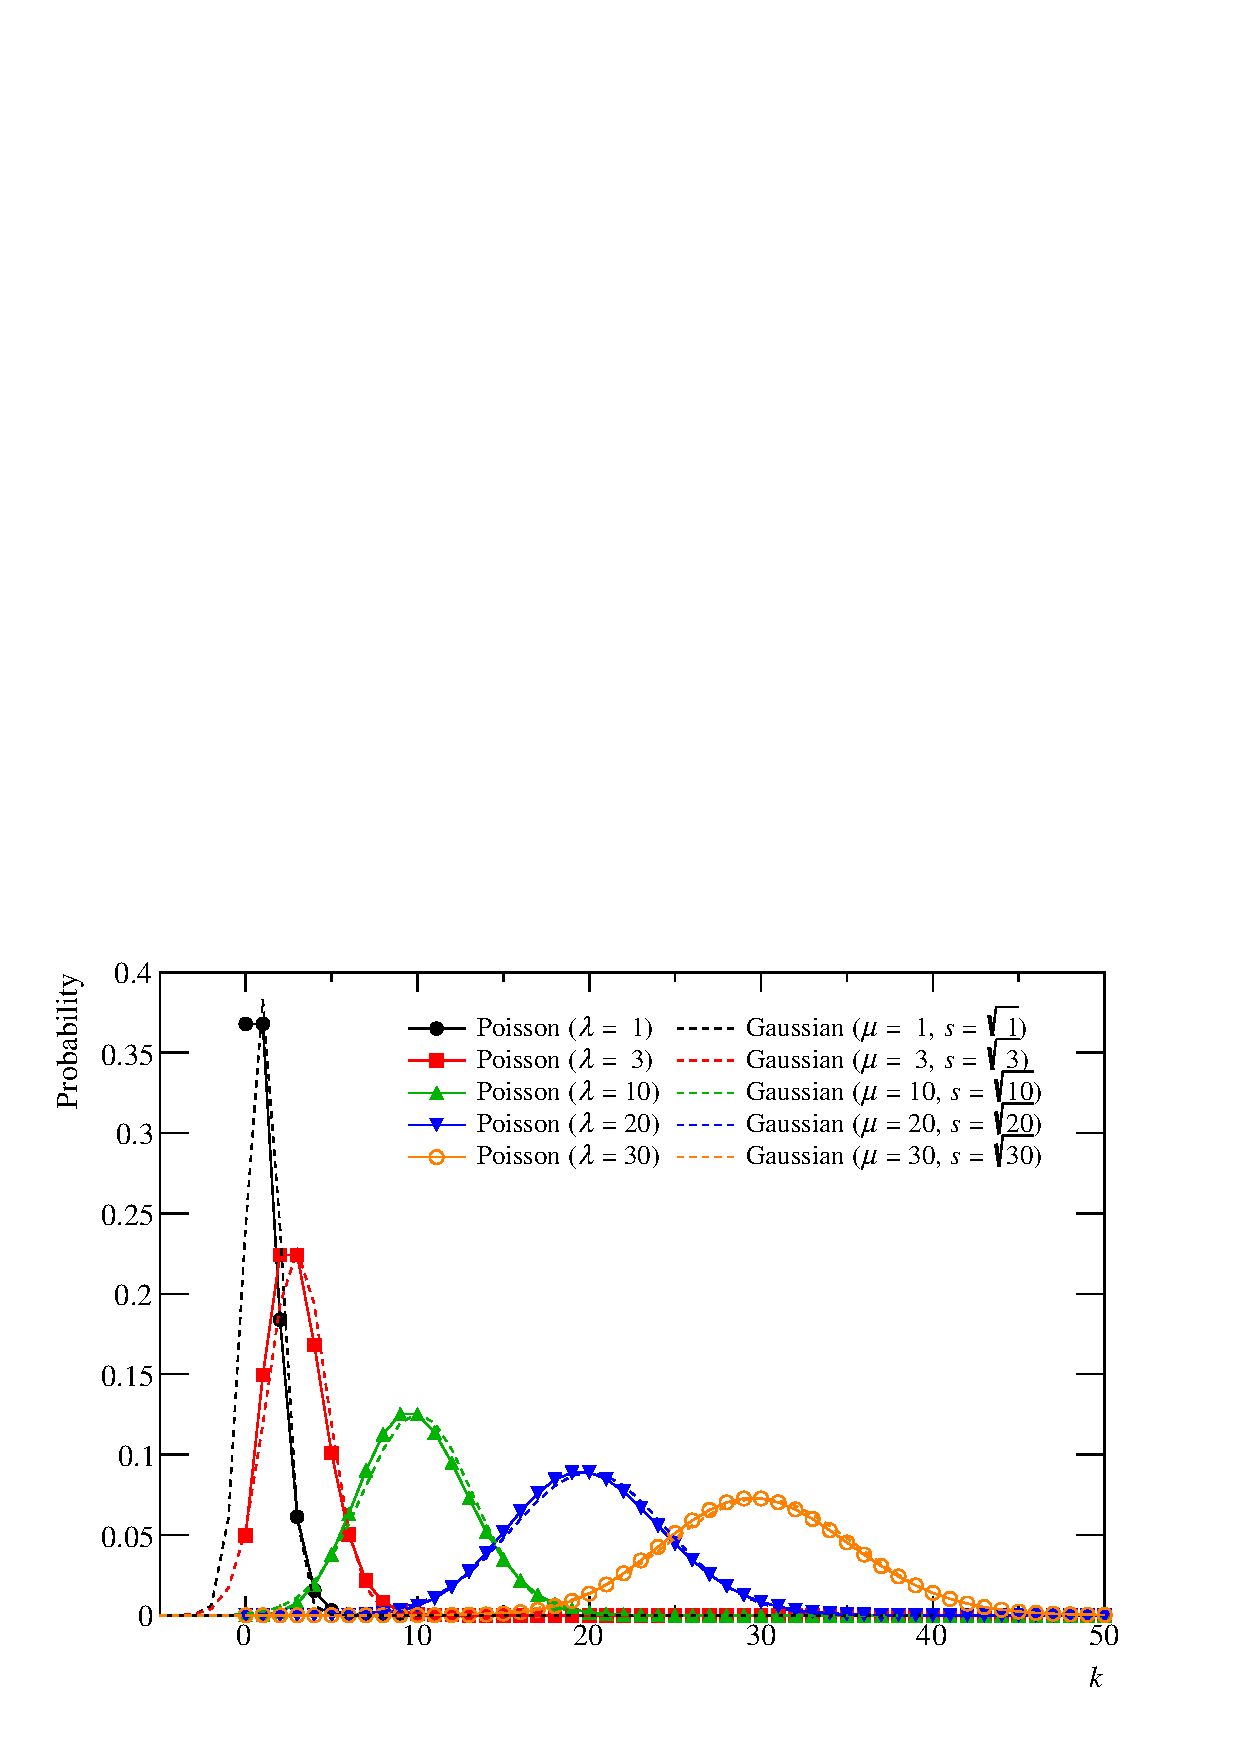
\includegraphics[width=12cm]{fig/Poisson.pdf}
  \caption{様々な平均値を持つポアソン分布と正規分布の比較}
  \label{fig_Poisson}
\end{figure}

\subsection{指数分布}
\subsection{二項分布}
\subsection{カイ二乗分布}

